\documentclass[11pt,a4paper]{article}
%%%%%%%%%%%%%%%%%%%%%%%%% Credit %%%%%%%%%%%%%%%%%%%%%%%%

% template ini dibuat oleh martin.manullang@if.itera.ac.id untuk dipergunakan oleh seluruh sivitas akademik itera.

%%%%%%%%%%%%%%%%%%%%%%%%% PACKAGE starts HERE %%%%%%%%%%%%%%%%%%%%%%%%
\usepackage{graphicx}
\usepackage{caption}
\captionsetup[figure]{name=Gambar}
\usepackage{tabulary}
% \usepackage{amsmath}
\usepackage{fancyhdr}
% \usepackage{amssymb}
% \usepackage{amsthm}
\usepackage{placeins}
% \usepackage{amsfonts}
\usepackage{graphicx}
\usepackage[all]{xy}
\usepackage{tikz}
\usepackage{verbatim}
\usepackage[left=2cm,right=2cm,top=3cm,bottom=2.5cm]{geometry}
\usepackage{hyperref}
\hypersetup{
    colorlinks,
    linkcolor={red!50!black},
    citecolor={blue!50!black},
    urlcolor={blue!80!black}
}
\usepackage{libertine}
\usepackage{libertinust1math}
\usepackage[T1]{fontenc}
\usepackage{inconsolata}

\usepackage{caption}
\usepackage{subcaption}
\usepackage{multirow}
\usepackage{psfrag}
\usepackage[T1]{fontenc}
\usepackage[scaled]{beramono}
% Enable inserting code into the document
\usepackage{listings}
\usepackage{xcolor} 
% custom color & style for listing
\definecolor{codegreen}{rgb}{0,0.6,0}
\definecolor{codegray}{rgb}{0.5,0.5,0.5}
\definecolor{codepurple}{rgb}{0.58,0,0.82}
\definecolor{backcolour}{rgb}{0.95,0.95,0.92}
\lstdefinestyle{mystyle}{
	backgroundcolor=\color{backcolour},   
	commentstyle=\color{green},
	keywordstyle=\color{codegreen},
	numberstyle=\tiny\color{codegray},
	stringstyle=\color{codepurple},
	basicstyle=\ttfamily\footnotesize,
	breakatwhitespace=false,         
	breaklines=true,                 
	captionpos=b,                    
	keepspaces=true,                 
	numbers=left,                    
	numbersep=5pt,                  
	showspaces=false,                
	showstringspaces=false,
	showtabs=false,                  
	tabsize=2
}
\lstset{style=mystyle}
\renewcommand{\lstlistingname}{Kode}
%%%%%%%%%%%%%%%%%%%%%%%%% PACKAGE ends HERE %%%%%%%%%%%%%%%%%%%%%%%%


%%%%%%%%%%%%%%%%%%%%%%%%% Data Diri %%%%%%%%%%%%%%%%%%%%%%%%
\newcommand{\stuid}{120140141}
\newcommand{\student}{\textbf{Bilhaq Avi Dewantara (\stuid{})}}
\newcommand{\course}{\textbf{Sistem Operasi (IF2223)}}
\newcommand{\assignment}{\textbf{02}} % tugas ke...

%%%%%%%%%%%%%%%%%%% using theorem style %%%%%%%%%%%%%%%%%%%%
\newtheorem{thm}{Theorem}
\newtheorem{lem}[thm]{Lemma}
\newtheorem{defn}[thm]{Definition}
\newtheorem{exa}[thm]{Example}
\newtheorem{rem}[thm]{Remark}
\newtheorem{coro}[thm]{Corollary}
\newtheorem{quest}{Question}[section]
%%%%%%%%%%%%%%%%%%%%%%%%%%%%%%%%%%%%%%%%
\usepackage{lipsum}%% a garbage package you don't need except to create examples.
\usepackage{fancyhdr}
\usepackage[ddmmyyyy]{datetime}
\pagestyle{fancy}
\lhead{ \student }
\rhead{ \thepage}
\cfoot{\textbf{Hands On 2: Synchronisation and Deadlock}} % ini untuk judul tugas
\renewcommand{\headrulewidth}{0.4pt}
\renewcommand{\footrulewidth}{0.4pt}

%%%%%%%%%%%%%%  Shortcut for usual set of numbers  %%%%%%%%%%%

\newcommand{\N}{\mathbb{N}}
\newcommand{\Z}{\mathbb{Z}}
\newcommand{\Q}{\mathbb{Q}}
\newcommand{\R}{\mathbb{R}}
\newcommand{\C}{\mathbb{C}}
\setlength\headheight{14pt}

%%%%%%%%%%%%%%%%%%%%%%%%%%%%%%%%%%%%%%%%%%%%%%%%%%%%%%%555

\begin{document}
\thispagestyle{empty}
\begin{center}
	
\includegraphics[scale = 0.15]{Figure1/ifitera-header.png}
	\vspace{0.1cm}
\end{center}
\noindent
% change font family for header section only
%{\fontfamily{LinuxLibertineT-OsF}\large\selectfont 
{\large
\rule{17cm}{0.2cm}\\[0.3cm]
Nama: \student \hfill Tugas Ke: \assignment\\[0.1cm]
Mata Kuliah: \course \hfill Tanggal: \today\\
\rule{17cm}{0.05cm}
\vspace{0.1cm}
}


%%%%%%%%%%%%%%%%%%%%%%%%%%%%%%%%%%%%%%%%%%%%% BODY DOCUMENT %%%%%%%%%%%%%%%%%%%%%%%%%%%%%%%%%%%%%%%%%%%%%
\section{Tujuan Hands On 2}
    Tujuan adanya Hands On kedua adalah untuk memahami bagaimana sistem bersinkronisasi dan permasalahan yang ada, serta juga memahami solusinya saat menjalankan critical section.
	Adapun beberapa implementasi yang diharuskan untun dipahami pada Hands On kedua ini antara lain : \textit{join} menggunakan semaphores, \textit{Binary Semaphores}, 
	\textit{Produces Consumer}, \textit{Reader/Writer Locks}, dan \textit{Dining Philosophers}.


\section{Fork/Join}
\subsection{Source Code}
\begin{lstlisting}[language=C]
	#include <stdio.h>
	#include <stdlib.h>
	#include <pthread.h>
	#include <unistd.h>

	#include "common.h"
	#include "common_threads.h"

	#ifdef linux
	#include <semaphore.h>
	#elif __APPLE__
	#include "zemaphore.h"
	#endif

	sem_t s;

	void *child(void *arg) {
	sleep(2);
	printf("child\n");
	Sem_post(&s); // signal here: child is done
	return NULL;
	}

	int main(int argc, char *argv[]) {
	Sem_init(&s, 0); 
	printf("parent: begin\n");
	pthread_t c;
	Pthread_create(&c, NULL, child, NULL);
	Sem_wait(&s); // wait here for child
	printf("parent: end\n");
	return 0;
	}
	\end{lstlisting}

\subsection{Output}
\begin{figure}[h]
	\centering
	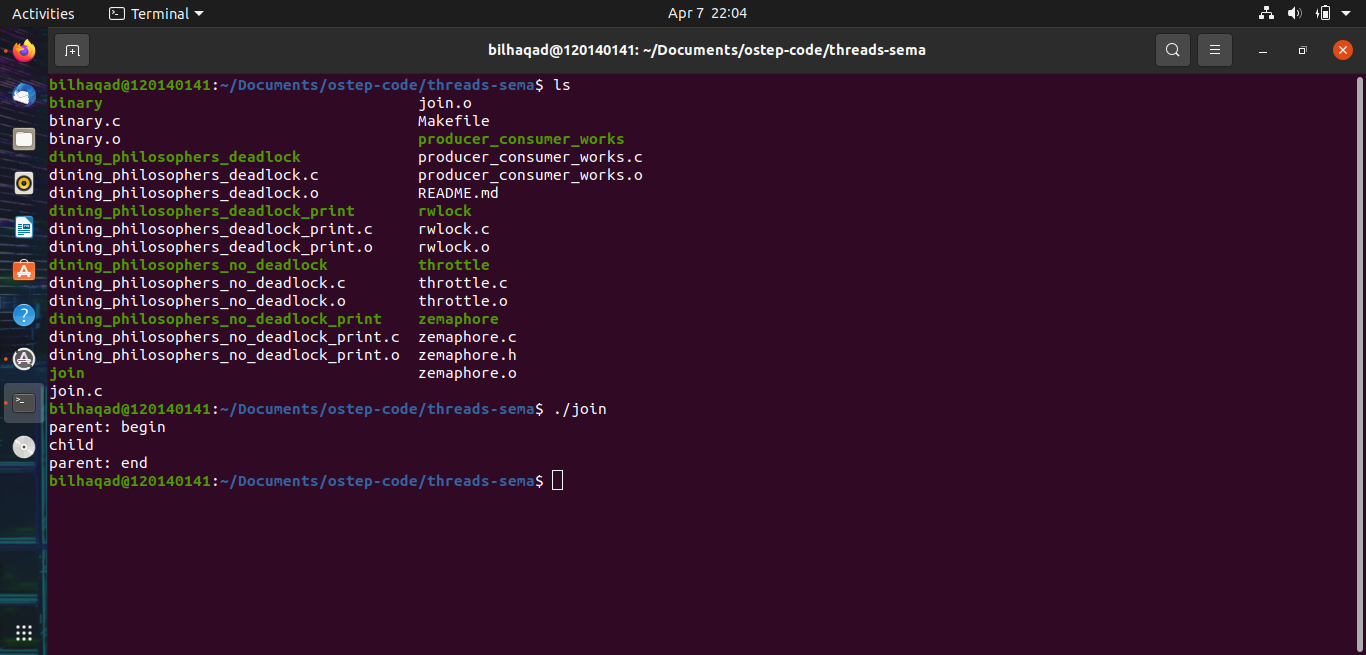
\includegraphics[width=0.8\textwidth]{Figure1/fork.png}
	\caption{\textit{Fork/Join}}
\end{figure}

\subsection{Penjelasan \textit{Fork/Join}}


\section{Binary Semaphores}
\subsection{Source Code}
\begin{lstlisting}[language=C]
	#include <stdio.h>
	#include <stdlib.h>
	#include <pthread.h>
	#include <unistd.h>

	#include "common.h"
	#include "common_threads.h"

	#ifdef linux
	#include <semaphore.h>
	#elif __APPLE__
	#include "zemaphore.h"
	#endif

	sem_t mutex;
	volatile int counter = 0;

	void *child(void *arg) {
		int i;
		for (i = 0; i < 10000000; i++) {
		Sem_wait(&mutex);
		counter++;
		Sem_post(&mutex);
		}
		return NULL;
	}

	int main(int argc, char *argv[]) {
		Sem_init(&mutex, 1); 
		pthread_t c1, c2;
		Pthread_create(&c1, NULL, child, NULL);
		Pthread_create(&c2, NULL, child, NULL);
		Pthread_join(c1, NULL);
		Pthread_join(c2, NULL);
		printf("result: %d (should be 20000000)\n", counter);
		return 0;
	}
\end{lstlisting}

\subsection{Output}
\begin{figure}[h]
	\centering
	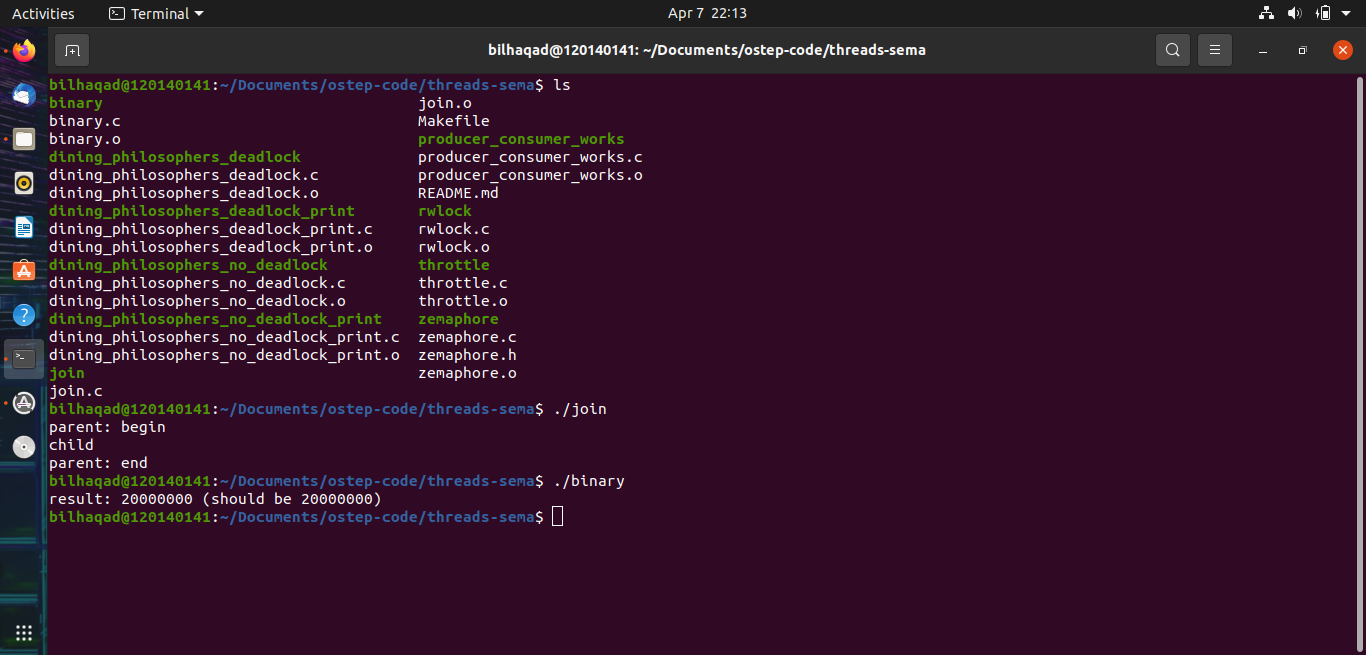
\includegraphics[width=0.8\textwidth]{Figure1/binary.png}
	\caption{\textit{Binary Semaphores}}
\end{figure}

\subsection{Penjelasan \textit{Binary Semaphores}}

\section{Producer/Consumer}
\subsection{Source Code}
\begin{lstlisting}[language=C]
	#include <stdio.h>
	#include <unistd.h>
	#include <assert.h>
	#include <pthread.h>
	#include <stdlib.h>

	#include "common.h"
	#include "common_threads.h"

	#ifdef linux
	#include <semaphore.h>
	#elif __APPLE__
	#include "zemaphore.h"
	#endif

	int max;
	int loops;
	int *buffer;

	int use  = 0;
	int fill = 0;

	sem_t empty;
	sem_t full;
	sem_t mutex;

	#define CMAX (10)
	int consumers = 1;

	void do_fill(int value) {
		buffer[fill] = value;
		fill++;
		if (fill == max)
		fill = 0;
	}

	int do_get() {
		int tmp = buffer[use];
		use++;
		if (use == max)
		use = 0;
		return tmp;
	}

	void *producer(void *arg) {
		int i;
		for (i = 0; i < loops; i++) {
		Sem_wait(&empty);
		Sem_wait(&mutex);
		do_fill(i);
		Sem_post(&mutex);
		Sem_post(&full);
		}

		// end case
		for (i = 0; i < consumers; i++) {
		Sem_wait(&empty);
		Sem_wait(&mutex);
		do_fill(-1);
		Sem_post(&mutex);
		Sem_post(&full);
		}

		return NULL;
	}
																				
	void *consumer(void *arg) {
		int tmp = 0;
		while (tmp != -1) {
		Sem_wait(&full);
		Sem_wait(&mutex);
		tmp = do_get();
		Sem_post(&mutex);
		Sem_post(&empty);
		printf("%lld %d\n", (long long int) arg, tmp);
		}
		return NULL;
	}

	int main(int argc, char *argv[]) {
		if (argc != 4) {
		fprintf(stderr, "usage: %s <buffersize> <loops> <consumers>\n", argv[0]);
		exit(1);
		}
		max   = atoi(argv[1]);
		loops = atoi(argv[2]);
		consumers = atoi(argv[3]);
		assert(consumers <= CMAX);

		buffer = (int *) malloc(max * sizeof(int));
		assert(buffer != NULL);
		int i;
		for (i = 0; i < max; i++) {
		buffer[i] = 0;
		}

		Sem_init(&empty, max); // max are empty 
		Sem_init(&full, 0);    // 0 are full
		Sem_init(&mutex, 1);   // mutex

		pthread_t pid, cid[CMAX];
		Pthread_create(&pid, NULL, producer, NULL); 
		for (i = 0; i < consumers; i++) {
		Pthread_create(&cid[i], NULL, consumer, (void *) (long long int) i); 
		}
		Pthread_join(pid, NULL); 
		for (i = 0; i < consumers; i++) {
		Pthread_join(cid[i], NULL); 
		}
		return 0;
	}
\end{lstlisting}
\subsection{Output}
\begin{figure}[h]
	\centering
	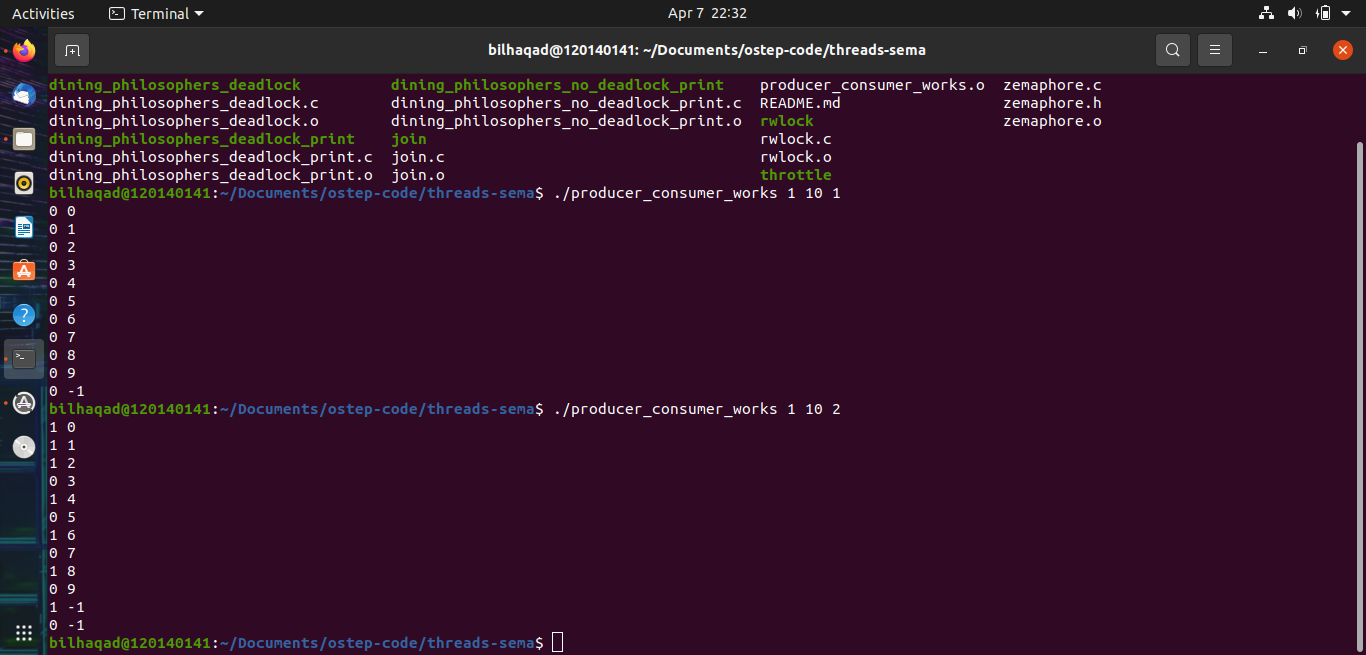
\includegraphics[width=0.8\textwidth]{Figure1/produce.png}
	\caption{\textit{Producer/Consumer}}
\end{figure}

\subsection{Penjelasan \textit{Producer/Consumer}}

\section{Reader/Writer Locks}
\subsection{Source Code}
\begin{lstlisting}[language=C]
	#include <stdio.h>
	#include <stdlib.h>
	#include <pthread.h>
	#include <unistd.h>
	
	#include "common.h"
	#include "common_threads.h"
	
	#ifdef linux
	#include <semaphore.h>
	#elif __APPLE__
	#include "zemaphore.h"
	#endif
	
	typedef struct _rwlock_t {
		sem_t writelock;
		sem_t lock;
		int readers;
	} rwlock_t;
	
	void rwlock_init(rwlock_t *lock) {
		lock->readers = 0;
		Sem_init(&lock->lock, 1); 
		Sem_init(&lock->writelock, 1); 
	}
	
	void rwlock_acquire_readlock(rwlock_t *lock) {
		Sem_wait(&lock->lock);
		lock->readers++;
		if (lock->readers == 1)
		Sem_wait(&lock->writelock);
		Sem_post(&lock->lock);
	}
	
	void rwlock_release_readlock(rwlock_t *lock) {
		Sem_wait(&lock->lock);
		lock->readers--;
		if (lock->readers == 0)
		Sem_post(&lock->writelock);
		Sem_post(&lock->lock);
	}
	
	void rwlock_acquire_writelock(rwlock_t *lock) {
		Sem_wait(&lock->writelock);
	}
	
	void rwlock_release_writelock(rwlock_t *lock) {
		Sem_post(&lock->writelock);
	}
	
	int read_loops;
	int write_loops;
	int counter = 0;
	
	rwlock_t mutex;
	
	void *reader(void *arg) {
		int i;
		int local = 0;
		for (i = 0; i < read_loops; i++) {
		rwlock_acquire_readlock(&mutex);
		local = counter;
		rwlock_release_readlock(&mutex);
		printf("read %d\n", local);
		}
		printf("read done: %d\n", local);
		return NULL;
	}
	
	void *writer(void *arg) {
		int i;
		for (i = 0; i < write_loops; i++) {
		rwlock_acquire_writelock(&mutex);
		counter++;
		rwlock_release_writelock(&mutex);
		}
		printf("write done\n");
		return NULL;
	}
	
	int main(int argc, char *argv[]) {
		if (argc != 3) {
		fprintf(stderr, "usage: rwlock readloops writeloops\n");
		exit(1);
		}
		read_loops = atoi(argv[1]);
		write_loops = atoi(argv[2]);
		
		rwlock_init(&mutex); 
		pthread_t c1, c2;
		Pthread_create(&c1, NULL, reader, NULL);
		Pthread_create(&c2, NULL, writer, NULL);
		Pthread_join(c1, NULL);
		Pthread_join(c2, NULL);
		printf("all done\n");
		return 0;
	}
\end{lstlisting}

\subsection{Output}
\begin{figure}[h]
	\centering
	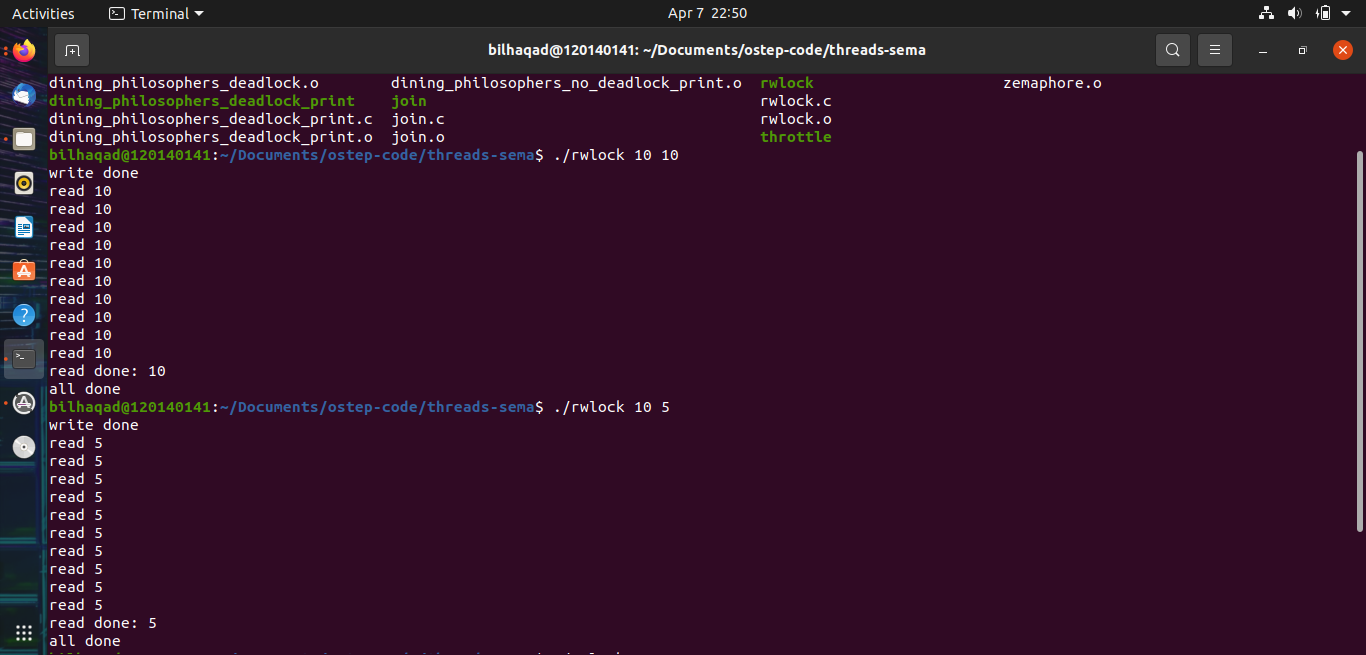
\includegraphics[width=0.8\textwidth]{Figure1/rwlock.png}
	\caption{\textit{Reader/Writer Locks}}
\end{figure}

\subsection{Penjelasan \textit{Reader/Writer Locks}}

\section{Dining Philosophers}
\subsection{Deadlock}
\subsubsection{Source Code}
\begin{lstlisting}{language=C}
	#include <stdio.h>
	#include <stdlib.h>
	#include <pthread.h>
	
	#include "common.h"
	#include "common_threads.h"
	
	#ifdef linux
	#include <semaphore.h>
	#elif __APPLE__
	#include "zemaphore.h"
	#endif
	
	typedef struct {
		int num_loops;
		int thread_id;
	} arg_t;
	
	sem_t forks[5];
	sem_t print_lock;
	
	void space(int s) {
		Sem_wait(&print_lock);
		int i;
		for (i = 0; i < s * 10; i++)
		printf(" ");
	}
	
	void space_end() {
		Sem_post(&print_lock);
	}
	
	int left(int p)  {
		return p;
	}
	
	int right(int p) {
		return (p + 1) % 5;
	}
	
	void get_forks(int p) {
		space(p); printf("%d: try %d\n", p, left(p)); space_end();
		Sem_wait(&forks[left(p)]);
		space(p); printf("%d: try %d\n", p, right(p)); space_end();
		Sem_wait(&forks[right(p)]);
	}
	
	void put_forks(int p) {
		Sem_post(&forks[left(p)]);
		Sem_post(&forks[right(p)]);
	}
	
	void think() {
		return;
	}
	
	void eat() {
		return;
	}
	
	void *philosopher(void *arg) {
		arg_t *args = (arg_t *) arg;
	
		space(args->thread_id); printf("%d: start\n", args->thread_id); space_end();
	
		int i;
		for (i = 0; i < args->num_loops; i++) {
		space(args->thread_id); printf("%d: think\n", args->thread_id); space_end();
		think();
		get_forks(args->thread_id);
		space(args->thread_id); printf("%d: eat\n", args->thread_id); space_end();
		eat();
		put_forks(args->thread_id);
		space(args->thread_id); printf("%d: done\n", args->thread_id); space_end();
		}
		return NULL;
	}
																				 
	int main(int argc, char *argv[]) {
		if (argc != 2) {
		fprintf(stderr, "usage: dining_philosophers <num_loops>\n");
		exit(1);
		}
		printf("dining: started\n");
		
		int i;
		for (i = 0; i < 5; i++) 
		Sem_init(&forks[i], 1);
		Sem_init(&print_lock, 1);
	
		pthread_t p[5];
		arg_t a[5];
		for (i = 0; i < 5; i++) {
		a[i].num_loops = atoi(argv[1]);
		a[i].thread_id = i;
		Pthread_create(&p[i], NULL, philosopher, &a[i]);
		}
	
		for (i = 0; i < 5; i++) 
		Pthread_join(p[i], NULL); 
	
		printf("dining: finished\n");
		return 0;
	}
\end{lstlisting}

\newpage
\subsubsection{Output}
\begin{figure}[h]
	\centering
	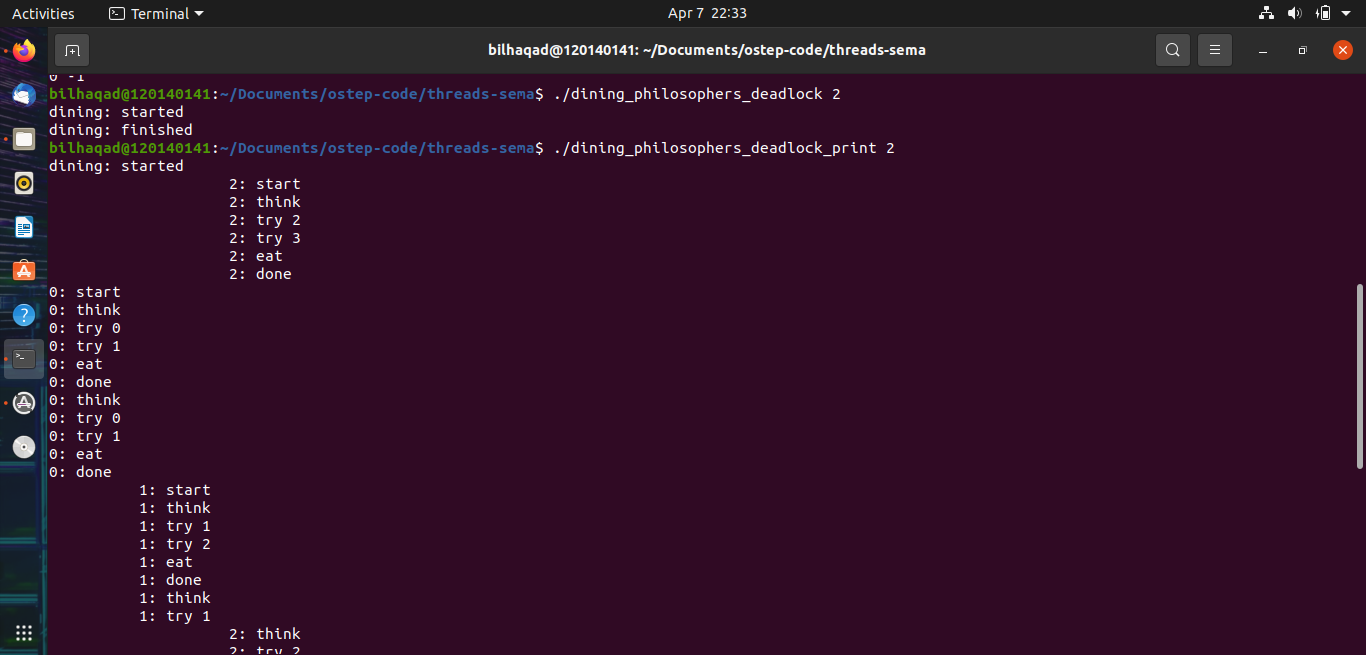
\includegraphics[width=0.8\textwidth]{Figure1/dining_deadlock1.png}
	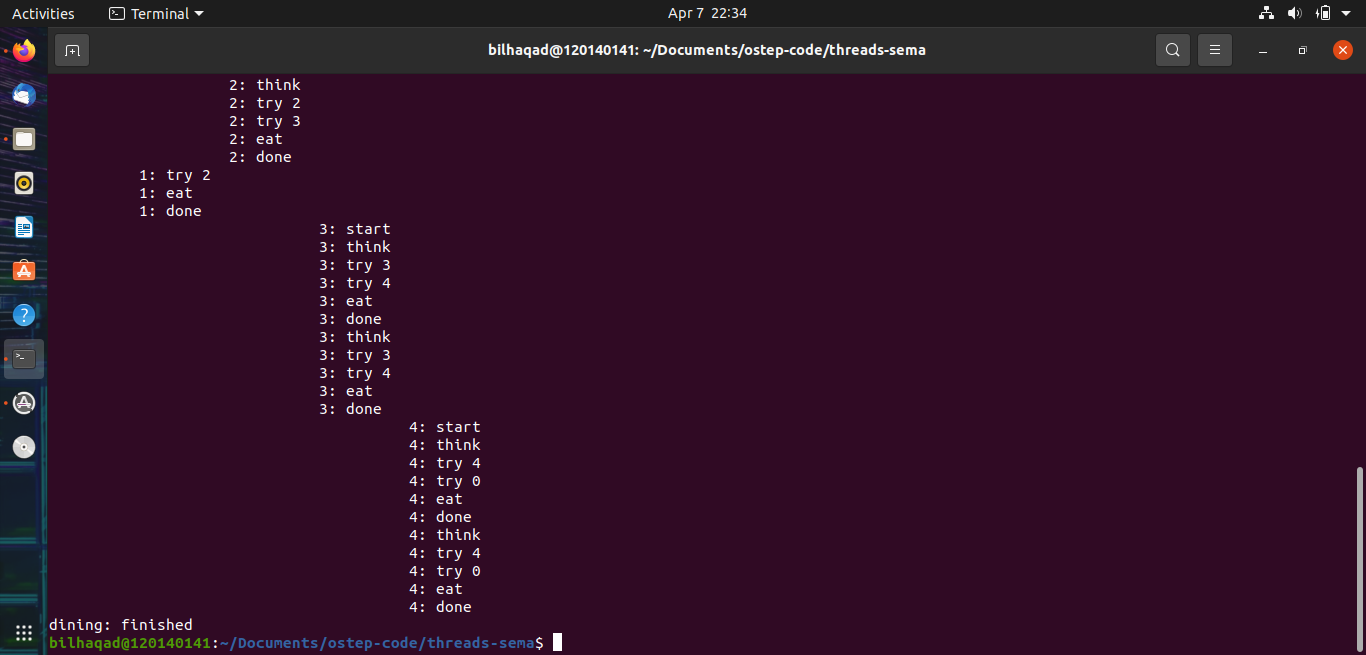
\includegraphics[width=0.8\textwidth]{Figure1/dining_deadlock2.png}
\end{figure}

\subsubsection{Penjelasan \textit{Dining Philosophers Deadlock}}

\newpage
\subsection{No Deadlock}
\subsubsection{Source Code}
\begin{lstlisting}[language=C]
	#include <stdio.h>
	#include <stdlib.h>
	#include <pthread.h>

	#include "common.h"
	#include "common_threads.h"

	#ifdef linux
	#include <semaphore.h>
	#elif __APPLE__
	#include "zemaphore.h"
	#endif

	typedef struct {
		int num_loops;
		int thread_id;
	} arg_t;

	sem_t forks[5];
	sem_t print_lock;

	void space(int s) {
		Sem_wait(&print_lock);
		int i;
		for (i = 0; i < s * 10; i++)
		printf(" ");
	}

	void space_end() {
		Sem_post(&print_lock);
	}

	int left(int p)  {
		return p;
	}

	int right(int p) {
		return (p + 1) % 5;
	}

	void get_forks(int p) {
		if (p == 4) {
		space(p); printf("4 try %d\n", right(p)); space_end();
		Sem_wait(&forks[right(p)]);
		space(p); printf("4 try %d\n", left(p)); space_end();
		Sem_wait(&forks[left(p)]);
		} else {
		space(p); printf("try %d\n", left(p)); space_end();
		Sem_wait(&forks[left(p)]);
		space(p); printf("try %d\n", right(p)); space_end();
		Sem_wait(&forks[right(p)]);
		}
	}

	void put_forks(int p) {
		Sem_post(&forks[left(p)]);
		Sem_post(&forks[right(p)]);
	}

	void think() {
		return;
	}

	void eat() {
		return;
	}

	void *philosopher(void *arg) {
		arg_t *args = (arg_t *) arg;

		space(args->thread_id); printf("%d: start\n", args->thread_id); space_end();

		int i;
		for (i = 0; i < args->num_loops; i++) {
		space(args->thread_id); printf("%d: think\n", args->thread_id); space_end();
		think();
		get_forks(args->thread_id);
		space(args->thread_id); printf("%d: eat\n", args->thread_id); space_end();
		eat();
		put_forks(args->thread_id);
		space(args->thread_id); printf("%d: done\n", args->thread_id); space_end();
		}
		return NULL;
	}
																				
	int main(int argc, char *argv[]) {
		if (argc != 2) {
		fprintf(stderr, "usage: dining_philosophers <num_loops>\n");
		exit(1);
		}
		printf("dining: started\n");
		
		int i;
		for (i = 0; i < 5; i++) 
		Sem_init(&forks[i], 1);
		Sem_init(&print_lock, 1);

		pthread_t p[5];
		arg_t a[5];
		for (i = 0; i < 5; i++) {
		a[i].num_loops = atoi(argv[1]);
		a[i].thread_id = i;
		Pthread_create(&p[i], NULL, philosopher, &a[i]);
		}

		for (i = 0; i < 5; i++) 
		Pthread_join(p[i], NULL); 

		printf("dining: finished\n");
		return 0;
	}
\end{lstlisting}

\newpage
\subsubsection{Output}
\begin{figure}[h]
	\centering
	\begin{subfigure}[b]{0.4\textwidth}
		\centering
		\def\svgwidth{\columnwidth}
		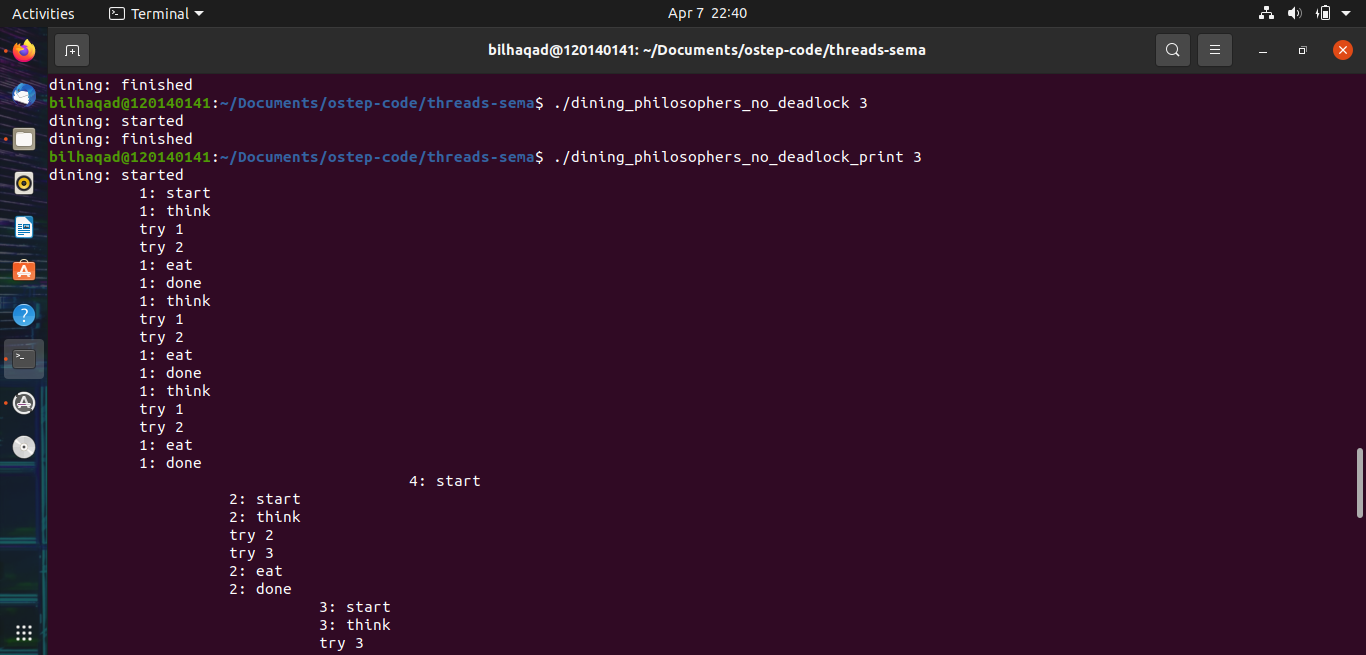
\includegraphics[width=1\textwidth]{Figure1/dining_nodeadlock1.png}
		\label{fig:nodeadlock1}
	\end{subfigure}
	\qquad %add desired spacing between images, e. g. ~, \quad, \qquad, \hfill etc. 
	%(or a blank line to force the subfigure onto a new line)
	\begin{subfigure}[b]{0.4\textwidth}
		\centering
		\def\svgwidth{\columnwidth}
		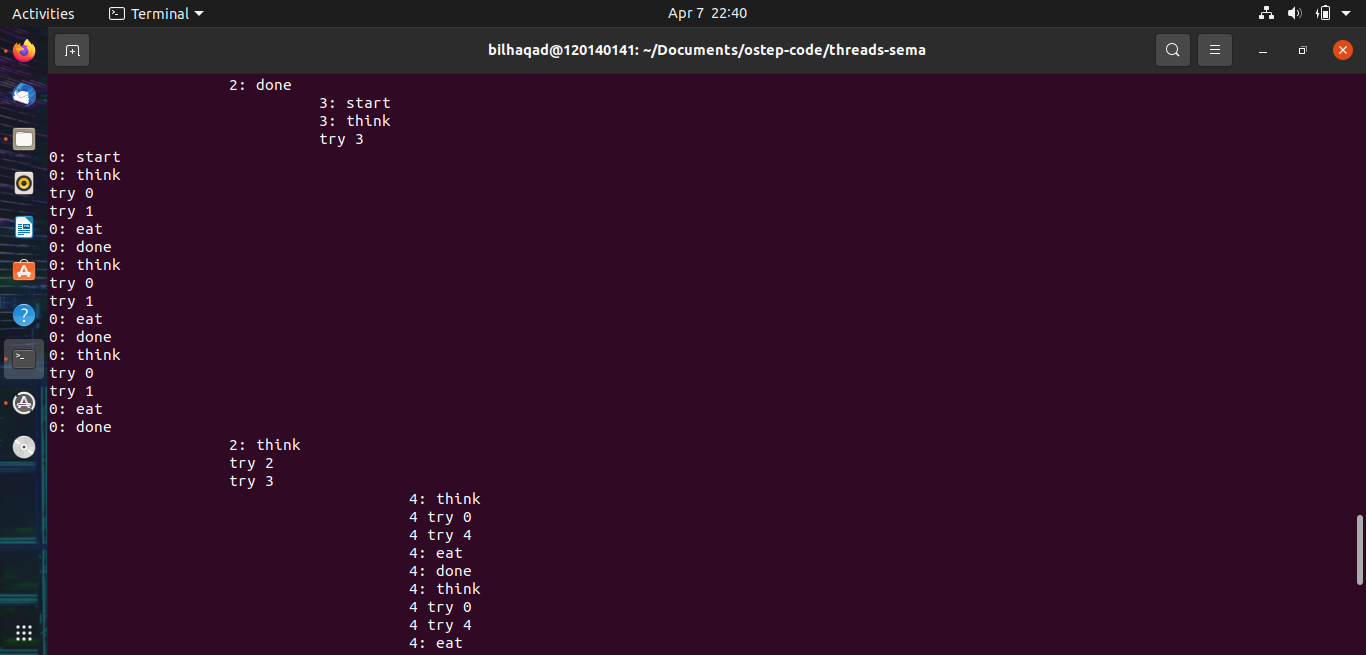
\includegraphics[width=1\textwidth]{Figure1/dining_nodeadlock2.png}
		\label{fig:nodeadlock2}
	\end{subfigure}
	\begin{subfigure}[b]{0.4\textwidth}
		\centering
		\def\svgwidth{\columnwidth}
		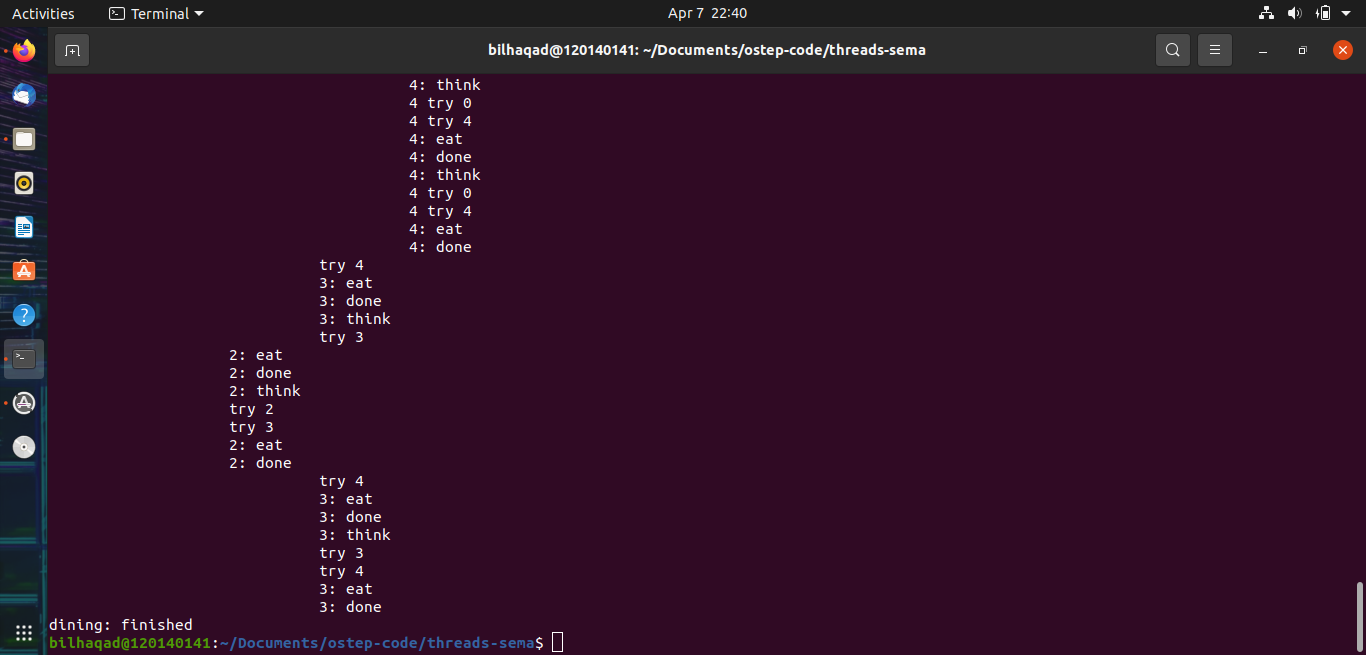
\includegraphics[width=1\textwidth]{Figure1/dining_nodeadlock3.png}
		\label{fig:nodeadlock3}
	\end{subfigure}
	\caption{Dining Philosophers No Deadlock}\label{fig:aug}
\end{figure}

\subsubsection{Penjelasan \textit{Dining Philosophers No Deadlock}}

\newpage
\section{Kesimpulan}
	Pada Hands On 1 ini yang saya dapatkan setelah menjalankannya ialah saya dapat mengenal sistem operasi linux
	khususnya Ubuntu 20.04 LTS ini meskipun hanya menggunakan Oracle VirtualBox. Selain itu, saya dapat mengetahui
	banyak hal dari tugas ini yaitu itu menggunakan konsep-konsep baru dan mengimplementasikannya pada terminal di linux.
	Dengan begitu, saya dapat menyelesaikan tugas ini sesuai dengan kemampuan yang saya miliki terutama menggunakan latex
	ini yang baru bagi saya, sehingga banyak sekali yang saya dapatkan dari tugas ini.
		
\section{Link GitHub}
	Link GitHub dari Hands On 2 ini : \href{https://github.com/BilhaqAD07/Sistem-Operasi.git}{Klik disini}


\newpage
\bibliographystyle{IEEEtran}
\bibliography{Referensi}
\end{document}